\documentclass[9pt]{beamer}

\usepackage{proof}
\usepackage{latexsym}
\usepackage{amsmath}
\usepackage{cmll}
\usepackage{mycommands-GAMES}
%\usepackage{mycommands}
\usepackage{xcolor}
\usepackage{colortbl}
%\usepackage{beamerthemeBoadilla}
%\usepackage{gslist}
%\usepackage{gsgraph}
%\usepackage{dgames_slides}
\usepackage{xspace}
\usepackage{wasysym}
\usepackage{graphicx}
\usepackage{wrapfig}
%\usepackage{ulem}

\sloppy

\definecolor{darkgreen}{rgb}{0,.3,0}
\definecolor{darkred}{rgb}{.5,0,0}
\definecolor{darkblue}{rgb}{0,0,.7}
\definecolor{darkvio}{rgb}{.5,0,.5}
\definecolor{darkorange}{rgb}{.8,0,.4}
\definecolor{lightgreen}{rgb}{0,.9,0}
\definecolor{itemblue}{rgb}{0,0,.4}
\definecolor{lightblue}{rgb}{0,0,.3}
\definecolor{bananamania}{rgb}{0.98, 0.91, 0.71}
\definecolor{black}{rgb}{0.0, 0.0, 0.0}

\renewcommand{\emph}[1]{{\color{blue} #1}}
\newcommand{\emphdb}[1]{{\color{darkblue} #1}}
\newcommand{\empha}[1]{{\color{darkgreen} #1}}
\newcommand{\emphb}[1]{{\color{darkvio} #1}}
\newcommand{\emphdr}[1]{{\color{darkred} #1}}
\newcommand{\emphdo}[1]{{\color{darkorange} #1}}
\newcommand{\emphbl}[1]{{\color{black} #1}}
\newcommand{\semitransp}[2][35]{\color{fg!#1}#2}

\newcommand{\yellow}[1]{{\color{yellow} #1}}
\newcommand{\white}[1]{{\color{white} #1}}
\newcommand{\violet}[1]{{\color{violet} #1}}
\newcommand{\teal}[1]{{\color{teal} #1}}
%\newcommand{\red}[1]{{\color{red} #1}}
\newcommand{\purple}[1]{{\color{purple} #1}}
\newcommand{\pink}[1]{{\color{pink} #1}}
\newcommand{\orange}[1]{{\color{orange} #1}}
\newcommand{\olive}[1]{{\color{olive} #1}}
\newcommand{\magenta}[1]{{\color{magenta} #1}}
\newcommand{\lime}[1]{{\color{lime} #1}}
\newcommand{\lightgray}[1]{{\color{lightgray} #1}}
\newcommand{\green}[1]{{\color{green} #1}}
\newcommand{\gray}[1]{{\color{gray} #1}}
\newcommand{\darkgray}[1]{{\color{darkgray} #1}}
\newcommand{\cyan}[1]{{\color{cyan} #1}}
\newcommand{\brown}[1]{{\color{brown} #1}}
%\newcommand{\blue}[1]{{\color{blue} #1}}
\newcommand{\black}[1]{{\color{black} #1}}

\newcommand{\bred}[1]{\colorbox{red!30}{#1}}
\newcommand{\bblue}[1]{\colorbox{cyan!30}{#1}}
\newcommand{\byellow}[1]{\colorbox{yellow!30}{#1}}
\newcommand{\bgreen}[1]{\colorbox{olive!30}{#1}}
\newcommand{\bmag}[1]{\colorbox{magenta!30}{#1}}
\newcommand{\bvio}[1]{\colorbox{violet!30}{#1}}

\usepackage{hyperref}
\hypersetup{
    colorlinks=true,
    linkcolor=blue,
    filecolor=magenta,      
    urlcolor=blue,
}


\newcommand{\seqb}[3]{#1: #2\lra #3}
\newcommand{\Pts}{\sf{PtS}}
\newcommand{\Bes}{\sf{BeS}}
\newcommand{\At}{\sf{At}}
\newcommand{\Atb}{\At_\bot}


\title[Playing with modalities]{Playing with modalities}
\author[Pimentel]{\emph{Elaine Pimentel (UCL)}\\
Carlos Olarte, Timo Lang\\
Robert Freiman, Chris Ferm\"uller
}
\institute[UCL]{\emph{FoSS SEMINAR}\\ October 30, 2024}
\date[FoSS]{
\includegraphics[scale=0.15]{../figs/Brighton}
}

\begin{document}

\maketitle

\section*{Motivation}

\begin{frame}{\only<1,2>{What is ``resource aware''?}\only<3,4>{What are ``modalities''?}\only<5>{In this talk:}}
\begin{itemize}
\item<1,2> Spent my PhD  \cyan{trying to figure it out}...
\item<2> ... but never through its \magenta{meaning}!
\end{itemize}

\begin{itemize}
\item<3,4> Proof theory
\item<4> Kripke structures
\end{itemize}

\only<5>{\pink{Dialogical games}: }
\begin{itemize}
\item<5>  for linear logic;
\item<5>  for modal logic.
\end{itemize}


\end{frame}

\section<presentation>*{Outline}

\begin{frame}{Outline}
\tableofcontents
\end{frame}
%\AtBeginSubsection[]
\AtBeginSection[]
{
\frame<handout:0>
{
\frametitle{Outline}
\tableofcontents[current,currentsubsection]
}
}


\section{Part I: Dialogical games for linear logic}

\begin{frame}{Game semantics \& LL}
\begin{columns}[T]
    \begin{column}{.4\textwidth}
    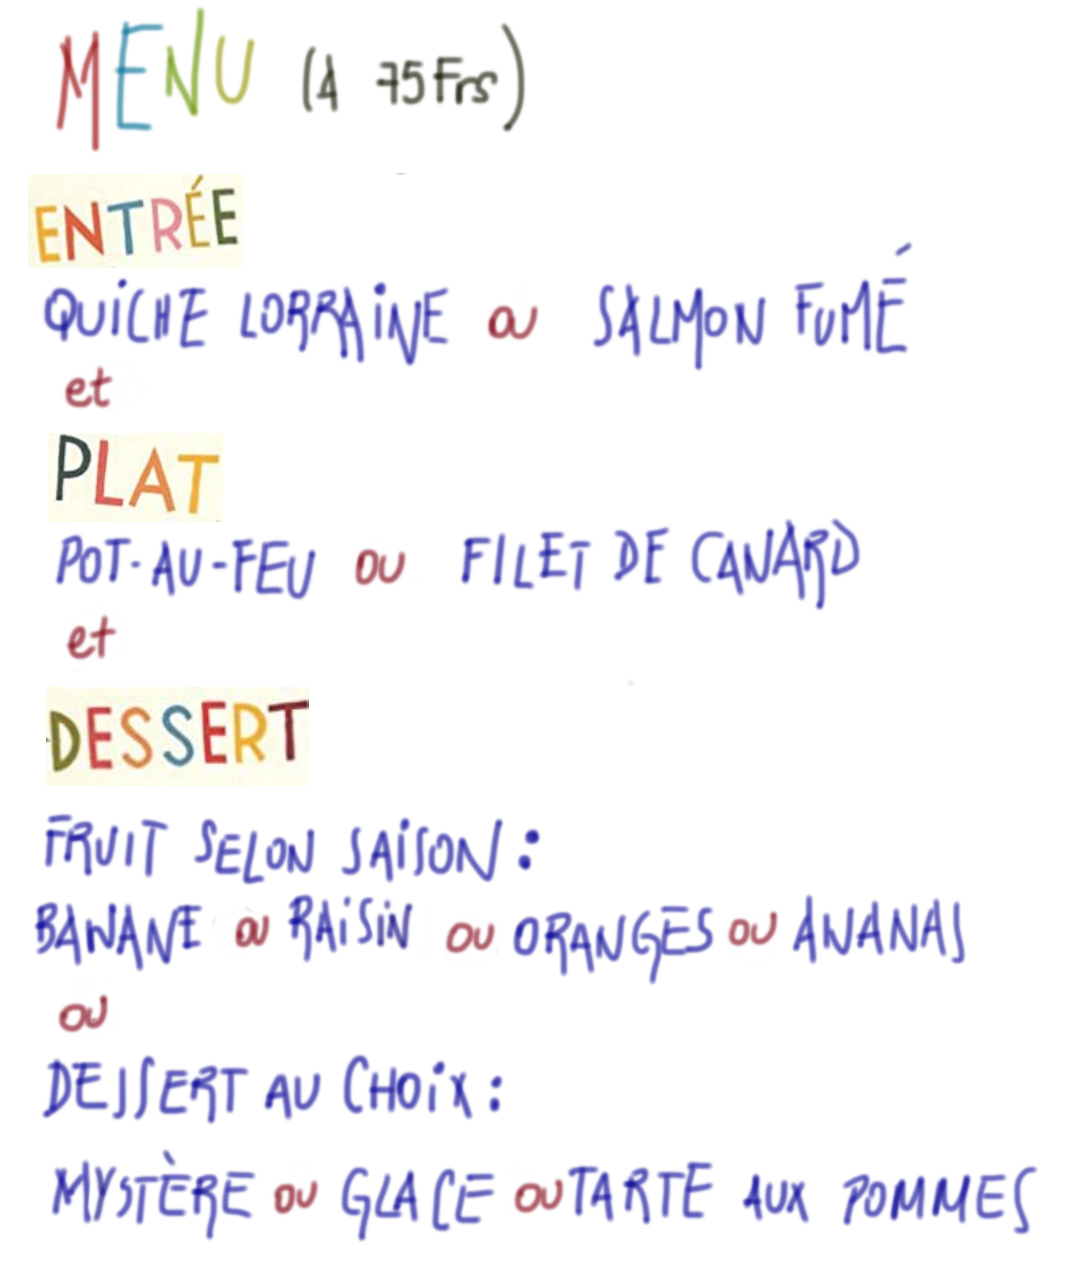
\includegraphics[scale=0.15]{../figs/menu1}
    \end{column}
    \begin{column}{.5\textwidth}
 \begin{itemize}
\item  \emph{Resource consciousness:} motivation usually remains \emphb{metaphorical}.

\item \emphdb{Gentzen's sequent calculus}  is a (the?) natural starting point
        for connecting  \emphdb{inference and resource consciousness}.

\item To \emphb{breathe life into the resource metaphor}, we need \emph{dynamics}\\[1ex]
       $\Longrightarrow$ \emphb{game semantics} for substructural sequent calculi. 
\item \empha{Our view of game semantics:} a \emphdo{playground} for illuminating specific 
intuitions underlying certain
proof systems.
\end{itemize}
    \end{column}
  \end{columns}
\end{frame}



\begin{frame}{Dialogues as foundations}


\begin{block}{Dialogues}
A Proponent~$\PP$ 
tries to defend a logically complex statement against attacks by
an Opponent~\OO. 
The dialogue \emphb{stepwise reduces complex assertions} to their components.	
\end{block} \pause

\XX/\YY\ stands for \PP/\OO\ {or} \OO/\PP\\[0.8ex]
%\begin{center}
\begin{tabular}{|c|c|c|}
\hline
\ statement by \XX\ \   &    attack by \YY   & defense by \XX  \\ 
\hline
\hline
$A \And B$ &\ \llll? or \rrr?  (\YY\ chooses) \ 
                           &\ $A$ or $B$, accordingly \ \\  \hline 
$A \Or B$   &    ?  &  $A$ or $B$ (\XX\ chooses) \\ \hline %*%\pause
$A \Impl B$  &      A             &        B             \\ \hline %*%\pause
% $\neg A$      &       A              &   (none)            \\ \hline %*%\pause
\end{tabular}

\vspace*{1ex}

\pause
\emph{Winning conditions for $\PP$:}

\vspace*{-0.2ex}
%\fbox{\parbox{60ex}{
\begin{description}
\item[W:] $\OO$ has already granted $\PP$'s {active formula}
\item[W$\f$:] $\OO$ has granted~$\f$
\end{description}
%}}

\emphdb{[Lorenzen'60]} attempted to \emph{\em{justify} constructive logic}. The completeness result w.r.t. LJ came much later \emphdb{[Felscher'85]}. 
  
\end{frame}

%\section{Linear logic}

\begin{frame}{The object-level}
\begin{center}
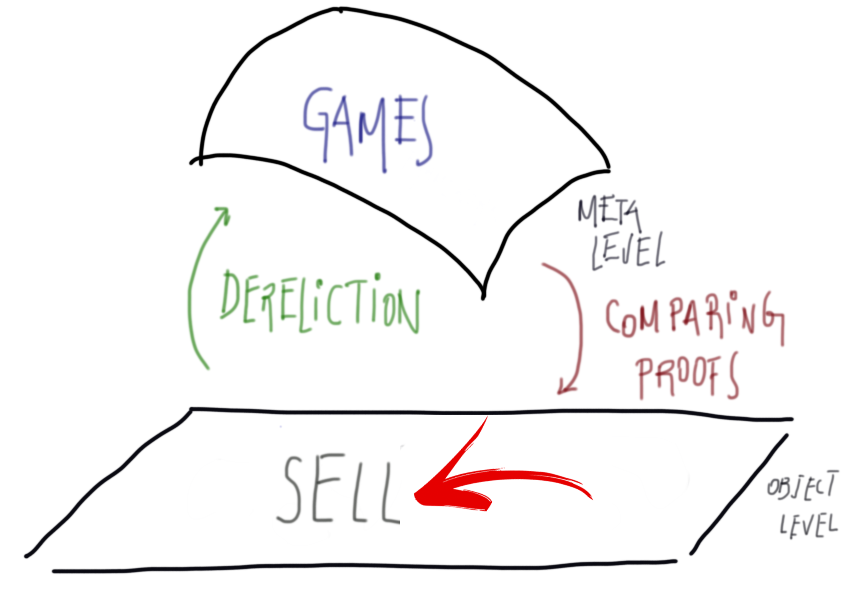
\includegraphics[scale=0.35]{../figs/LF9}
\end{center}
\end{frame}


\begin{frame}{Affine intuitionistic multiplicative additive LL ($\aIMALL$)}
\small{$$\begin{array}{c}
\hline\mbox{Sequent System for }\aIMALL\\\hline\\
\emph{\infer[\tensor_R]{\Delta_1, \Delta_2 \lra A \tensor B}
{\Delta_1 \lra A & \Delta_2 \lra B}
\quad 
\infer[\with_R]{\Gamma \lra A \with B}
{\Gamma \lra A & \Gamma \lra B}
\quad \infer[\lolli_R]{\Gamma \lra A \lolli B}{\Gamma, A \lra B}}
\\\\
 \infer[\tensor_L]{\Gamma, A \tensor B \lra C}
{\Gamma, A, B \lra C} 
\quad
\infer[\lolli_L]{\Delta_1, \Delta_2, A \lolli B \lra C}
{\Delta_1 \lra A & \Delta_2, B \lra C}
\quad
 \infer[\with_{L_i}]{\Gamma, A_1 \with A_2 \lra B}
{\Gamma, A_i\lra B} 
\\\\
\infer[\oplus_L]{\Gamma, A \oplus B \lra C}
{\Gamma, A \lra C & \Gamma, B \lra C}
\quad 
\infer[\oplus_{R_i}]{\Gamma \lra A_1 \oplus A_2}{\Gamma \lra A_i}
\\\\
\emph{\infer[I]{\Gamma,p \lra p}{} 
 \qquad
\infer[\one_R]{\Gamma \lra \one}{}
\qquad 
\infer[\zero_L]{ \Gamma,\zero\lra A}{}}
\end{array}
$$}
\end{frame}


%\section{A game model of branching}
\begin{frame}{The meta-level}
\begin{center}
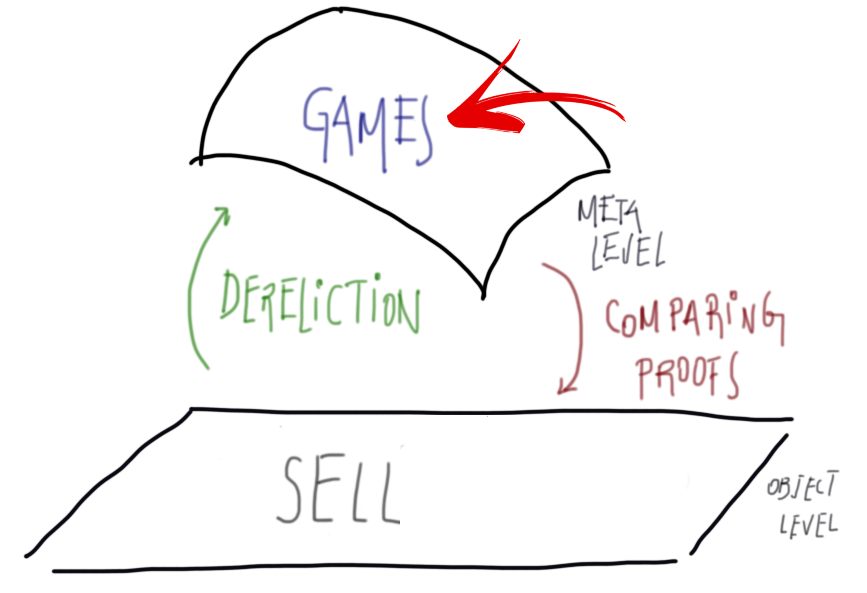
\includegraphics[scale=0.35]{../figs/LF10}
\end{center}
\end{frame}


\begin{frame}{The game for $\aIMALL$ \emphdb{[Ferm\"{u}ller,Lang17]}}
\begin{itemize}
	\item \emph{Formulas} are seen as \emphb{resources} that can be build from atomic propositions, units $\zero, \one$  and the constructors $ \otimes, \with, \oplus,\limp$

	\xitem \emph{States}: multisets of sequents of the form $\Gamma \lra F$
	\xitem Two players: $\PP$ and \OO. Player   $\PP$ starts the game and selects  a sequent $S$ from the current state.
	\xitem The game proceeds in rounds with two possible succ. states: 
	\[
\begin{array}{llllll}
{(1)} &G\cup\{S\}\quad&\leadsto&\quad G\cup\{S'\} & \qquad &\\
{(2)} &G\cup\{S\}\quad&\leadsto&\quad G\cup\{S_1\}\cup\{S_2\} & \qquad &
\end{array}
\]
\xitem  $\PP$ chooses a sequent $S$ among the current game state, a principal formula in $S$ and a matching rule instance $r$. 
\xitem $\PP$  acts as the \emphdo{scheduler} of the game.
\end{itemize}
\end{frame}


\begin{frame}{Multiplicative vs Additive}
\empha{Both are (right) branching rules}:
 \[
 \infer[\with_R]{\Gamma \lra A \with B}
{\Gamma \lra A & \Gamma \lra B}
\qquad
\infer[\tensor_R]{\Gamma_1, \Gamma_2 \lra A \tensor B}
{\Gamma_1 \lra A & \Gamma_2 \lra B}
 \]
 \emphb{However}, the intended meaning is different:

\begin{itemize}
 \item \emphdr{$A \with B$}: $\PP$ must be prepared to play either $A$ or $B$ (\OO\ choice) but \emph{only one game}  is actually played. 
 \item \emphdr{$A \otimes B$}: \emph{both} subgames,   $A$ and $B$ must be played and $\PP$ must win both. % to win the $A\otimes B$ game. 

\end{itemize}
\pause
\begin{block}{Branching structure}
Both definitions (a single or a parallel game) are equivalent:  \empha{the existence of winning strategies for $\PP$ remains the same}. 

\emph{However, semantically, they provide different viewpoints of the connectives.}
\end{block}
\end{frame}


\begin{frame}{The game for $\aIMALL$}
\begin{overlayarea}{\textwidth}{5cm}
\only<1>{
\[
\infer[\oplus_{R_1}]{p, q\oplus r\lra (p\otimes q)\oplus(p\otimes r)}{}
\]
}
\only<2>{
\[
\infer[\oplus_{R_1}]{p, q\oplus r\lra (p\otimes q)\oplus(p\otimes r)}
{\infer[\otimes_R]{p, q\oplus r\lra (p\otimes q)}{}}
\]
}
\only<3>{
\[
\infer[\oplus_{R_1}]{p, q\oplus r\lra (p\otimes q)\oplus(p\otimes r)}
{\infer[\otimes_R]{p, q\oplus r\lra (p\otimes q)}
{\deduce{p\lra p}{\blue{\smiley}}&
\deduce{q\oplus r\lra q}{}}}
\]
}
\only<4>{
\[
\infer[\oplus_{R_1}]{p, q\oplus r\lra (p\otimes q)\oplus(p\otimes r)}
{\infer[\otimes_R]{p, q\oplus r\lra (p\otimes q)}
{\deduce{p\lra p}{\blue{\smiley}}&
\infer[\oplus_L]{q\oplus r\lra q}
{\deduce{q\lra q}{\blue{\smiley}}&
}}}
\]
}
\only<5>{
\[
\infer[\oplus_{R_1}]{p, q\oplus r\lra (p\otimes q)\oplus(p\otimes r)}
{\infer[\otimes_R]{p, q\oplus r\lra (p\otimes q)}
{\deduce{p\lra p}{\blue{\smiley}}&
\infer[\oplus_L]{q\oplus r\lra q}
{\deduce{q\lra q}{\blue{\smiley}}&
\deduce{r\lra q}{\red{\frownie}}}}}
\]
}
\only<6>{
\[
\infer[\oplus_{L}]{p, q\oplus r\lra (p\otimes q)\oplus(p\otimes r)}
{\infer[\oplus_{R_1}]{p, q\lra (p\otimes q)\oplus(p\otimes r)}
{\infer[\otimes_R]{p, q\lra (p\otimes q)}
{\deduce{p\lra p}{\blue{\smiley}}&
\deduce{q\lra q}{\blue{\smiley}}}}&
\deduce{p,r\lra (p\otimes q)\oplus(p\otimes r)}{}}
\]
}
\only<7>{
\[
\infer[\oplus_{L}]{p, q\oplus r\lra (p\otimes q)\oplus(p\otimes r)}
{\deduce{p, q\lra (p\otimes q)\oplus(p\otimes r)}{} &
\infer[\oplus_{R_2}]{p,r\lra (p\otimes q)\oplus(p\otimes r)}
{\infer[\otimes_R]{p,r\lra p\otimes r}
{\deduce{p\lra p}{\blue{\smiley}}&
\deduce{r\lra r}{\blue{\smiley}}}}}
\]
}
\only<8->{
\[
\infer[\oplus_{L}]{p, q\oplus r\lra (p\otimes q)\oplus(p\otimes r)}
{\infer[\oplus_{R_1}]{p, q\lra (p\otimes q)\oplus(p\otimes r)}
{\infer[\otimes_R]{p, q\lra (p\otimes q)}
{\deduce{p\lra p}{\blue{\smiley}}&
\deduce{q\lra q}{\blue{\smiley}}}}&
\infer[\oplus_{R_2}]{p,r\lra (p\otimes q)\oplus(p\otimes r)}
{\infer[\otimes_R]{p,r\lra p\otimes r}
{\deduce{p\lra p}{\blue{\smiley}}&
\deduce{r\lra r}{\blue{\smiley}}}}}
\]
}
%\only<9>{
%\begin{block}{Plays and strategies}
%
%A \emph{play} of \GAIMALL on a game state $H$ is a sequence $H_1,H_2,\ldots,H_n$ of game states, where each $H_{i+1}$ arises by playing one round on $H_i$.
%
% A \emph{strategy} (for \PP) on a game state $H$ is defined as a function telling \I how to move in any given state.
% 
% A strategy on $H$ is a \emph{winning strategy} if all plays following it eventually reach a winning state.
%Notation: $\wins{}{\GAIMALL} H$.
%% if $\PP$ has a w.s. on the game state $H$. 
%\end{block}
%}
\end{overlayarea}
\end{frame}



\begin{frame}{Lafont's menu revisited}
\only<1>{
\begin{center}
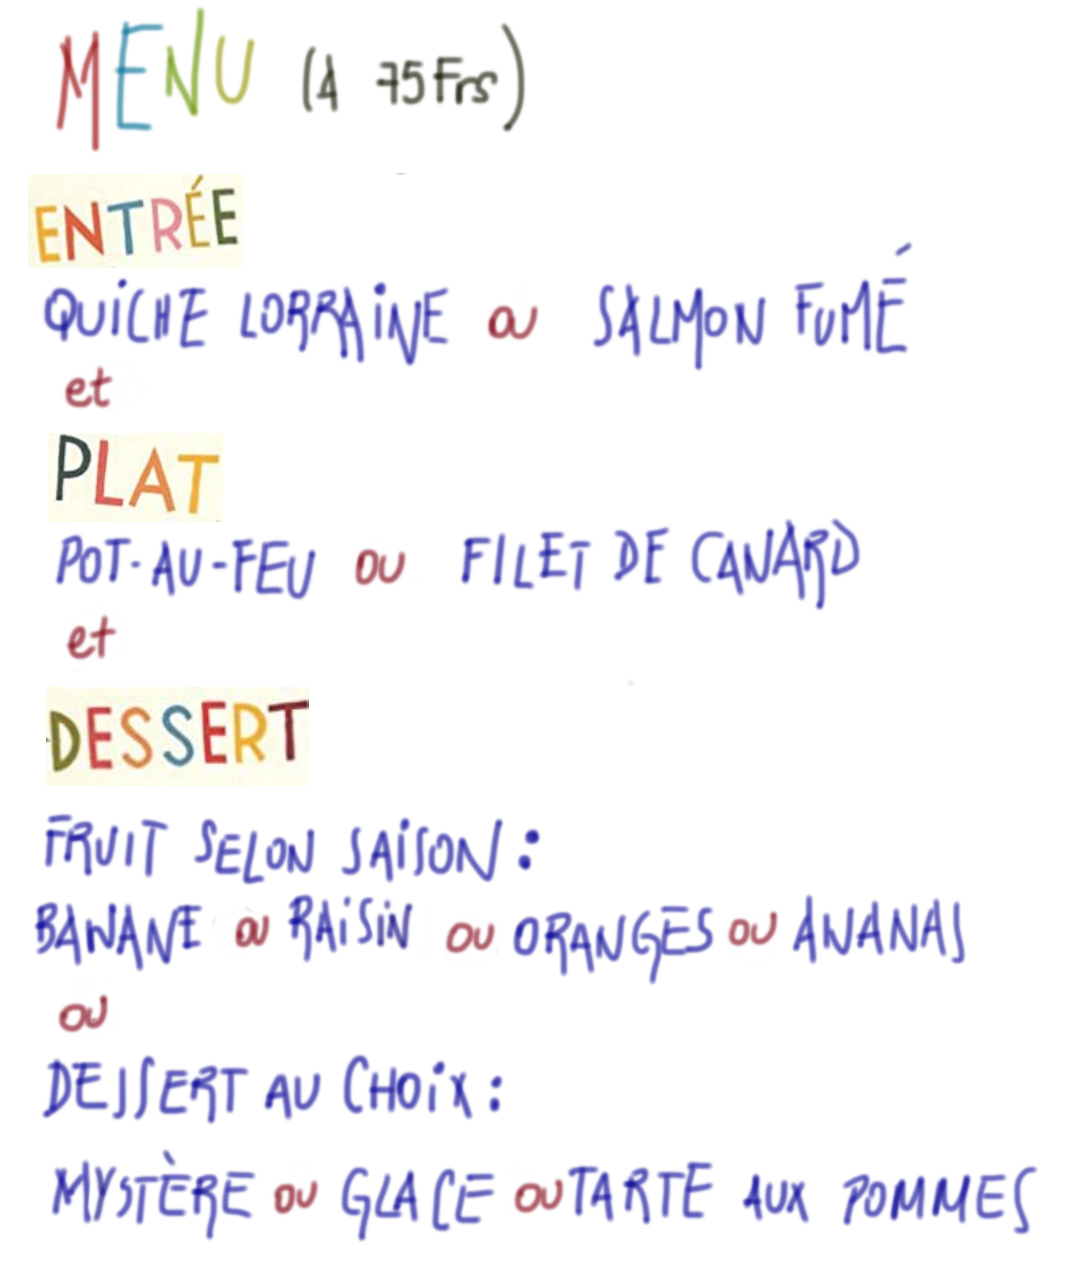
\includegraphics[scale=0.18]{../figs/menu1}
\end{center}}
\only<2>{
\begin{center}
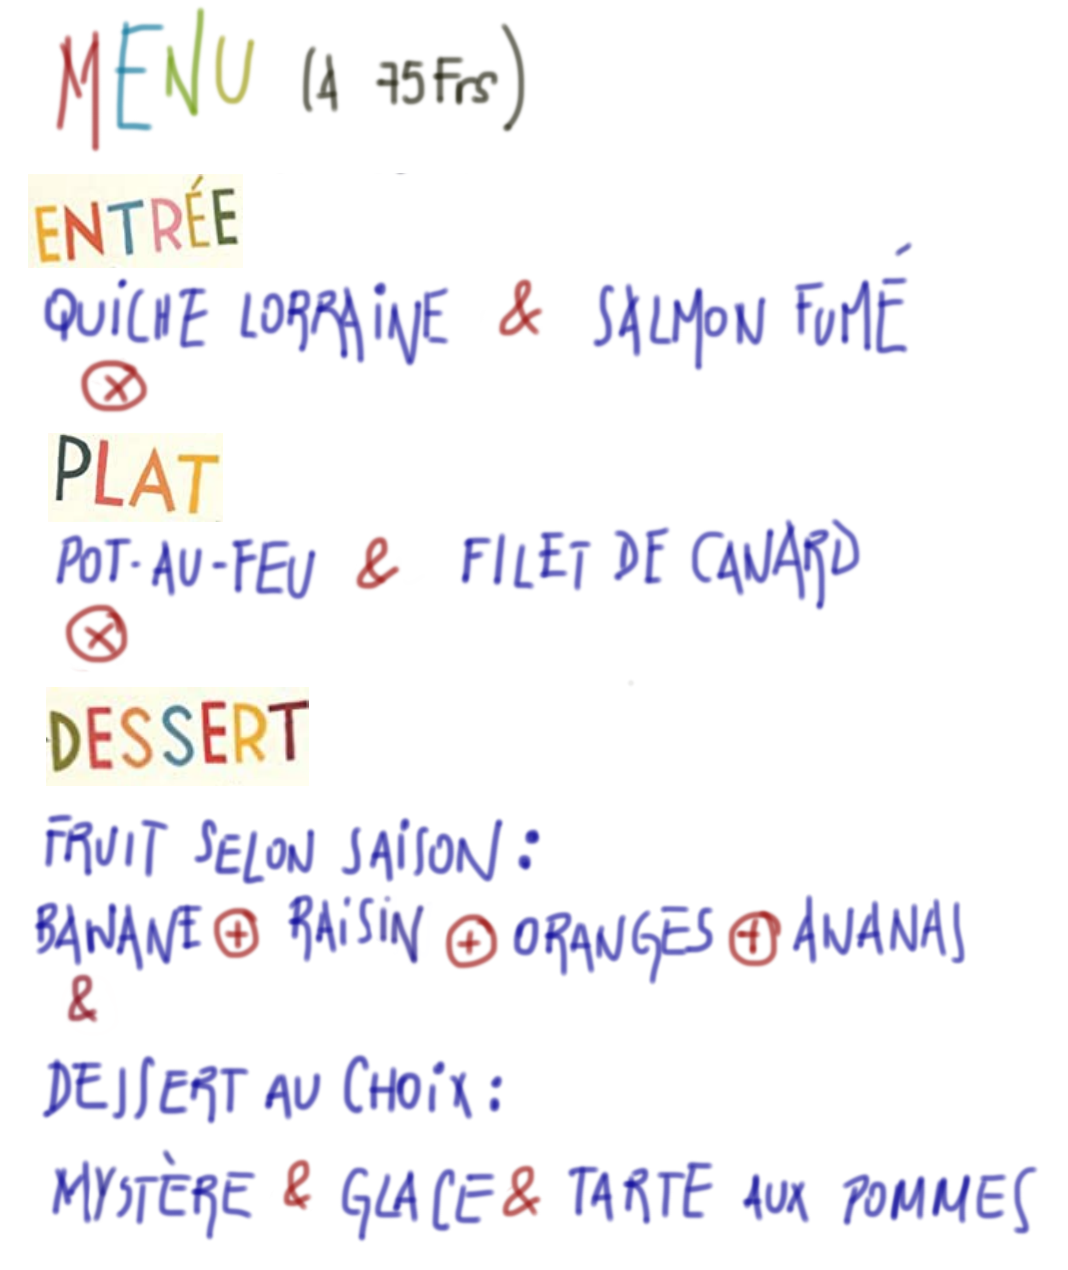
\includegraphics[scale=0.18]{../figs/menu}
\end{center}}
\end{frame}

\begin{frame}{Results}

\begin{block}{Independency}
$\wins{}{\GAIMALL}\{S_1,\ldots,S_n\}\quad\iff \quad\text{for all $i\leq n$, }\wins{}{\GAIMALL}S_i$
\end{block}
\bigskip 
\begin{block}{Adequacy for $\GAIMALL$}
Let $S$ be a sequent. Then 
$\wins{}{\GAIMALL}S\quad\iff\quad\vdash_\aIMALL S$
\end{block}

\end{frame}

%\section{Adding costs}

\begin{frame}{Intended meaning}
\begin{center}
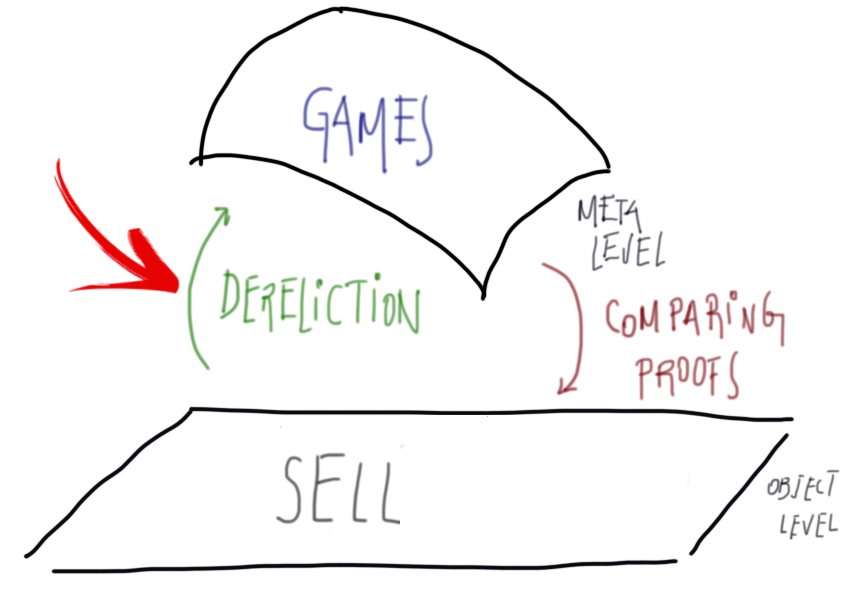
\includegraphics[scale=0.35]{../figs/LF12}
\end{center}
\end{frame}

\frame{
\frametitle{Subexponentials [Danos,Joinet,Schellinx'93]}
\only<1>{Exponentials in ILL:
 \[
  \begin{array}{c}
  \infer[\bang_L]{\Gamma, \blue{\bang A} \lra C }{\Gamma,\blue{A} \lra C }\qquad
  \infer[\bang_R]{\bang A_1, \ldots, \bang A_n \lra \blue{\bang A} }
  {\bang A_1, \ldots, \bang A_n \lra  \blue{A} }
  \end{array}
 \]
}
\only<2>{Sub-exponentials in ILL:
 \[
  \begin{array}{c}
  \infer[\nbang{a}_L]{\Gamma, \blue{\nbang{a} A} \lra C }{\Gamma,\blue{A} \lra C }\qquad
  \infer[\nbang{a}_R \mbox{, provided }a \preceq a_i]{\nbang{a_1} A_1, \ldots, \nbang{a_n} A_n \lra \blue{\nbang{a} A} }
  {\nbang{a_1} A_1, \ldots, \nbang{a_n} A_n \lra  \blue{A} }
  \end{array}
 \]
}
\only<3>{Sub-exponentials in ILL:
 \[
  \begin{array}{c}
  \infer[\nbang{a}_L]{\Gamma, \blue{\nbang{a} A} \lra C }{\Gamma,\blue{A} \lra C }\qquad
  \infer[\nbang{a}_R \mbox{, provided }a \preceq a_i]{\nbang{a_1} A_1, \ldots, \nbang{a_n} A_n \lra \blue{\nbang{a} A} }
  {\nbang{a_1} A_1, \ldots, \nbang{a_n} A_n \lra  \blue{A} }
  \end{array}
 \]
Then:
\begin{block}{}
$
\nbang{a}A\not\equiv \nbang{b} A
$ for \blue{any} $a\not= b$.
 \end{block}
}
}



\begin{frame}{Assumptions plus cost -- system $\aIMALLR$}
Augment assumptions with \emph{costs}, where assumptions are formulas occurring \emph{negatively} on sequents. 



\[ \infer[\nbang{a}_L,\;a\in\real^+]{\Gamma, \nbang{a} A \lra C }{\Gamma, \nbang{a} A,A \lra C }\]

\end{frame}


\begin{frame}{The game $\GAIMALLR$ [Lang,Olarte,Pimentel,Ferm\"{u}ller'19]}
\begin{itemize}
\item \emph{States}:  tuples $(H,b)$, where $H$ is a finite multiset of $\real^+$-valued sequents and $b\in\real$ is a \emphdo{budget}.
\item \emph{Rounds}:  the successor state is determined according to rules that fit one of the two following schemes:

$
\begin{array}{lllll}
{(1)} &(G\cup\{S\},b)&\quad\leadsto\quad&  \quad (G\cup\{S'\},b') & \\
{(2)} &(G\cup\{S\},b)&\quad\leadsto\quad&  \quad (G\cup\{S^1\}\cup\{S^2\},b)
\end{array}
$
\xitem Depending on the $r$, the round proceeds as follows:
\begin{enumerate}
\item If the rule $r$ is not $\nbang{}_L$, then the game proceeds as before, with budget $b$.
\item \emphdo{Budget decrease:} $\nbang{}_L$ with premise $S'$ and principal formula $\nbang{a}A$, then the game proceeds in the game state $(G\cup\{S'\},b-a)$.
\item \emph{To win the game:} non negative final budget.
\end{enumerate}
\end{itemize}
%\pause
%\begin{block}{Winning states} A \emph{winning state} (for \I) is a game state $(H,b)$ such that all $S\in H$ are initial sequents of $\aIMALLR$ and $b\geq 0$. $\wins{}{\GAIMALLR}(H,b)$: \textit{The budget~$b$ suffices to win the game $H$.} 
%\end{block}
\end{frame}

%\begin{frame}{Example}
%Consider the state $
%(\{\nbang{1}p,\vnbang{3}q\lra p\tensor q\},5) 
%$. 
%\begin{itemize} 
%\xitem In a first move, $\PP$ picks $p\tensor q$ and, by $\tensor_R$, she  finds a partition of the premises not prefixed with~$\nbang{}$. 
%\xitem The only such premise here is $\vnbang{3}q$, and $\PP$ decides that it goes to the right premise of $\tensor_R$. 
%\xitem So by {\bf parallelism}, the new state is
%$
%(\{(\nbang{1}p\lra p),(\nbang{1}p,\vnbang{3}q\lra q)\},5)
%$. 
%\xitem She now chooses to pick $\nbang{1}p$ of the first component and, by {\bf budget decrease}, her budget decreases  and the next  state is 
%$
%(\{(\nbang{1}p,p\lra p),(\nbang{1}p,\vnbang{3}q\lra q)\},4)
%$. 
%\xitem 
%Now $\PP$ picks $\vnbang{3}q$  leading to
%$
%(\{(\nbang{1}p,p\lra p),(\nbang{1}p,q\lra q)\},1)
%$. 
%\xitem Since both components are inital sequents and  $budget \geq 0$, this is a winning state for $\PP$.
%\end{itemize}
%\end{frame}


%\begin{frame}{Results}
%\begin{block}{Weak adequacy for $\GAIMALLR$}
%\label{theorem:adeq2}
%Let $S$ be a sequent. Then 
%\[\exists b\left(\wins{}{\GAIMALLR}(S,b)\right)\quad\iff\quad\vdash_{\aIMALLR} S\]
%\end{block} 
%
%\begin{block}
%{Quasi-independency of subgames in $\GAIMALLR$}
%\label{lemma:independency2}
%\noindent $\wins{}{\GAIMALLR}(\{S_1,\ldots,S_n\},b)$ if and only if
%\noindent $\exists b_1,\ldots,b_n\geq 0$  s.t. $\sum_{i=1}^n b_i\leq b$  and for all $i\leq n$,  $\wins{}{\GAIMALLR}(S_i,b_i)$.  
%\end{block}
%\end{frame}

\begin{frame}{Properties}
\begin{center}
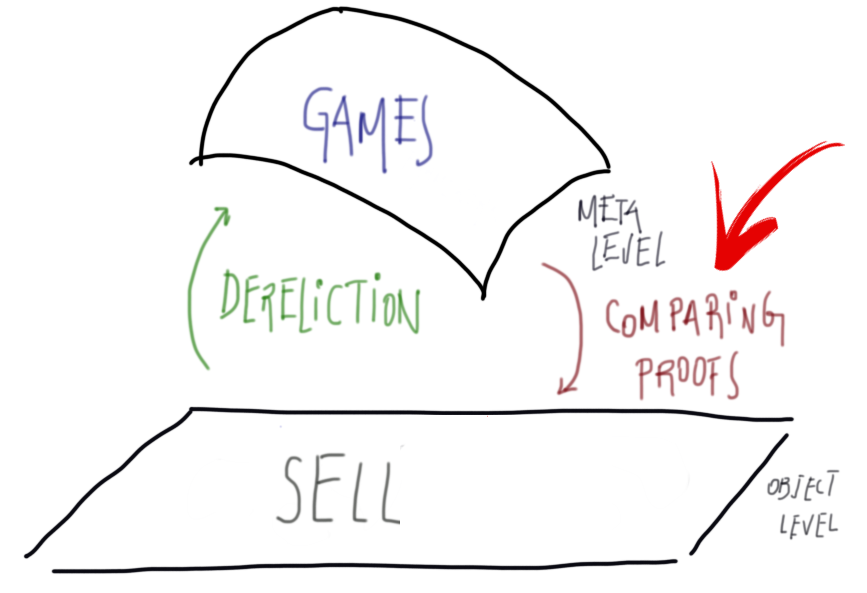
\includegraphics[scale=0.35]{../figs/LF11}
\end{center}
\end{frame}


\begin{frame}{Labelled system $\laIMALLR$}
\begin{itemize}
\item \emph{Weak adequacy}:  information about the budget $b$ is lost in the proof theoretic representation.
\item  In other words, the game $\GAIMALLR$ is more expressive than the calculus $\aIMALLR$.
\xitem To overcome this mismatch: a  labelled extension of $\aIMALLR$. 
\item A $\laIMALLR$-proof is build from labelled sequents 
$$\emphdr{b:}\;\Gamma\lra A$$ 
where $\Gamma\lra A$ is a $\aIMALLR$ sequent and $b\in\real^+$.
\end{itemize}
\end{frame}

\begin{frame}{Sequent rules for $\laIMALLR$}
$
\begin{array}{c}
\hline\mbox{Labelled sequent system for }\laIMALLR\\\hline\\
\infer[\tensor_R]{\emphdr{a+b:}\;\nbang{}\Gamma,\Delta_1, \Delta_2 \lra A\tensor B}
{\emphdr{a:}\;\nbang{}\Gamma,\Delta_1 \lra A & \emphdr{b:}\;\nbang{}\Gamma,\Delta_2 \lra B}
\quad
\infer[\with_R]{\emphdr{\max\{a,b\}:}\;\Gamma \lra A \with B}
{\emphdr{a:}\;\Gamma \lra A & \emphdr{b:}\;\Gamma \lra B}
\\\\
\infer[\nbang{}_L]{\emphdr{a+c:}\;\Gamma,\nbang{a}A\lra C}{\emphdr{c:}\;\Gamma,\nbang{a}A,A\lra C}
\\\\
  \infer[I\;\emphdr{b\geq 0}]{\emphdr{b:}\;\Gamma,p \lra p}{} 
 \quad
\infer[\one_R\;\emphdr{b\geq 0}]{\emphdr{b:}\;\Gamma \lra \one}{}
\quad 
\infer[\zero_L\;\emphdr{b\geq 0}]{\emphdr{b:}\; \Gamma,\zero\lra A}{}
\end{array}
$
\end{frame}


\begin{frame}{Example}
\begin{quote}
\empha{You have white and black socks in a drawer in a completely dark room. How many socks do you have to take out blindly to be sure of having a matching pair? }
\end{quote} \pause

\bigskip 
\begin{minipage}[0.2\textheight]{\textwidth}
\begin{columns}[T]
\begin{column}{0.8\textwidth}
\begin{itemize}
\item Matching pair: $(w\tensor w)\oplus(b\tensor b)$; 
\item Act of drawing a random sock: $\nbang{1}(w\oplus b)$. 
\end{itemize}
\end{column}
\begin{column}{0.2\textwidth}

\includegraphics[scale=0.5]{../figs/socks}
\end{column}
\end{columns}
\end{minipage} \pause

\begin{quote}
\emphdr{What is the smallest $n$ s.t. $\emphdr{n:}\;\nbang{1}(w\oplus b)\lra (w\tensor w)\oplus(b\tensor b)$ is provable?}
\end{quote} \pause
The answer, of course, is $3$: 

\resizebox{\textwidth}{!}{
$
\infer=[3\times\nbang{}_L]{\emphdr{3:}\;\nbang{1}(w\oplus b)\lra F}{
 \infer[\oplus_L]{\emphdr{0:}\;\nbang{1}(w\oplus b), w\oplus b, w\oplus b, w\oplus b\lra F}{
  \infer[\oplus_L]{\emphdr{0:}\;\nbang{1}(w\oplus b), w, w\oplus b, w\oplus b\lra F}{
   \infer[\oplus_L]{\emphdr{0:}\;\nbang{1}(w\oplus b), w, w, w\oplus b\lra F}{
   \infer=[\otimes_R, I]{\emphdr{0:}\;\nbang{1}(w\oplus b), w, w, w\oplus b\lra w\tensor w}{}
   }
   &
   \infer[\oplus_L]{\emphdr{0:}\;\nbang{1}(w\oplus b), w, b, w\oplus b\lra F}{
    \infer[\oplus_R]{\emphdr{0:}\;\nbang{1}(w\oplus b), w, b, w\lra F}{\infer=[\otimes_R,I]{\emphdr{0:}\;\nbang{1}(w\oplus b), w, b, w\lra (w\tensor w)}{}}
    &
    \infer{\emphdr{0:}\;\nbang{1}(w\oplus b), w, b, b\lra F}{\infer=[\otimes_R,I]{\emphdr{0:}\;\nbang{1}(w\oplus b), w, b, b\lra b\tensor b}{}}
   }
  }
  &
  \deduce{\pr}{}
 }
}
$
}
Game theoretically, $\PP$ must be prepared for any of the choices of \OO\ when she decides to select $w\oplus b$ (on the left). \end{frame}

\begin{frame}{Example}
A printer costs \$500 and produces copies for \$0.1. I want to make 2 copies. Which is the budget needed?\pause
\[
\emphdr{b:}\;  \nbang{500}(\nbang{0.1}C)\lra C\otimes C
\]
\pause
\[
\begin{array}{ccc}
\infer[\nbang{500}]{\emphdr{500.20:}\;  \nbang{500}(\nbang{0.1}C)\lra C\otimes C}
{\infer=[\nbang{0.10}]{\emphdr{0.20:}\;  \nbang{0.1}C\lra C\otimes C}
{\infer=[\otimes,\init]{\emphdr{0:}\;  C,C\lra C\otimes C}{}}} 
&\qquad&
\infer=[\nbang{500}]{\emphdr{1,000.20:}\;  \nbang{500}(\nbang{0.1}C)\lra C\otimes C}
{\infer=[\nbang{0.10}]{\emphdr{0.20:}\;  \nbang{0.1}C,\nbang{0.1}C\lra C\otimes C}
{\infer=[\otimes,\init]{\emphdr{0:}\;  C,C\lra C\otimes C}{}}} \\
\\
\mbox{\cyan{\underline{Reasonable strategy}:} } & & \mbox{\magenta{\underline{Stupid strategy}:} }\\
\mbox{Buy one printer, } & & \mbox{Buy two printers,} \\
\mbox{make 2 copies out of it.} & & \mbox{make one copy in each.}
\end{array}
\]

\end{frame}



\begin{frame}{Results}
%\begin{theorem}[strong adequacy for $\GAIMALLR$]
%\[\wins{}{\GAIMALLR}(\{\Gamma\lra A\},b)\quad\iff\quad\vdash_{\laIMALLR} \emphdr{b:}\; \Gamma\lra A\]
%\end{theorem} 
\begin{theorem}
Given a $\aIMALLR$-proof $\pr$ of a sequent $S$,  there exists a smallest budget with $\costs{\pr}$  that suffices to win the game $\GAIMALLR$ on $S$ when following the strategy corresponding to $\pr$.
\end{theorem}

\begin{block}{Spectrum}
$\spec{S}:=\{\costs{\pr}\mid\text{$\pr$ is an $\aIMALLR$-proof of $S$}\}$.
\end{block}
\begin{theorem}
If $\vdash_{\aIMALLR}\Gamma\lra A$, then $\spec{\Gamma\lra A}$ has a least element. In other words, there is a smallest $b$ such that $\vdash_{\laIMALLR}\Gamma\lra_b A$.
\end{theorem}
\end{frame}

%\section{The cost of cut}
\begin{frame}{Cut-elimination}
 $\aIMALLR$ inherits the admissibility of the following cut rule from~$\SELL$:
\[
\infer[cut]{\nbang{}\Gamma,\Delta_1,\Delta_2\lra C}
	{ \nbang{}\Gamma,\Delta_1\lra A &
	\nbang{}\Gamma,\Delta_2,A\lra C
	}
\] 
\emphdo{Note:} Remember that bangs occur \empha{negatively} only.
\pause
\begin{theorem}\label{thm:cutAdm}
For $f(a,b)=a+b$, the following cut rule is admissible in $\laIMALLR$:
\[
\infer[cut_\ell]{\emphdr{f(a,b):}\;\nbang{}\Gamma,\Delta_1,\Delta_2\lra C}
	{\emphdr{a:}\; \nbang{}\Gamma,\Delta_1\lra A &
	\emphdr{b:}\;\nbang{}\Gamma,\Delta_2,A\lra C
	}
\]
Moreover, whenever $cut_\ell$ is admissible w.r.t. $f:\real^+\times\real^+ \to \real^+$, then $a+b\leq f(a,b)$.
\end{theorem}
\end{frame}

\begin{frame}{What if we add exponentials to succedents?}
\begin{overlayarea}{\textwidth}{7cm}
\only<1->{
\[
\infer{\emphdr{b:}\;\Gamma\lra \nbang{a} A}{\emphdr{b:}\;\Gamma^{\preceq{a}}\lra A}
\]}
\only<2->{\emph{Cut-elimination FAILS!!}
\begin{theorem}\label{thm:impossible} There is no function $f:\real^+\times \real^+\rightarrow\real^+$ such that the rule
\[
\infer[cut]{\emphdr{f(a,b):}\;\nbang{}\Gamma,\Delta_1,\Delta_2\lra C}
	{\emphdr{a:}\; \nbang{}\Gamma,\Delta_1\lra A &
	\emphdr{b:}\;\nbang{}\Gamma,\Delta_2,A\lra C
	}
\]
is admissible in $\laIMALLR$.
\end{theorem}
}
\only<3->{
\begin{proof} Take

$\emphdr{a:}\; \nbang{1/k}p\lra\nbang{1/k}p^{\otimes (k\cdot a)}$

$\emphdr{b:}\; \nbang{1/k}p^{\otimes (k\cdot a)}\lra p^{\otimes(k\cdot k\cdot a\cdot b)} 
$ 

$ \emphdr{k.a.b:}\;\nbang{1/k}p\lra p^{\otimes(k\cdot k\cdot a\cdot b)}
$
\end{proof}
}
\end{overlayarea}
\end{frame}


%\section{Extensions and examples}

\begin{frame}{Generalizing the notion of cost [Bistarelli et al. 06]}
\begin{overlayarea}{\textwidth}{8cm}
\only<1-3>{
\begin{block}{The big picture}
Interpret prices and costs as elements of an algebraic structure:
\begin{itemize}
	\item \emph{compare}: when a cost/budget is better.
	\item \emph{combine}: how to accumulate costs/budgets
\end{itemize}
\end{block} }
\only<4->{
\begin{block}{The bigger picture}
Interpret prices and costs as elements of an algebraic structure:
\begin{itemize}
	\item \emph{compare}: when a cost/budget is better.
	\item \emph{combine}: how to accumulate costs/budgets
	\item \emph{split}: how to divide costs/budgets
\end{itemize}
\end{block} }
\only<2-3>{
\begin{center}
\begin{tabular}{lcl}
\emphdr{Absorptive semirings} &=&  top element ($a\leq 1$) plus\\
($a_1\times a_2\leq a_i$) && tropical semirings (comm. sem. $+$-idep.) or\\
& &  dioids or \\
&&  distributive partially ordered monoids.
\end{tabular}
\end{center}}
\only<3>{
\emphdr{Idea:}
$\langle A, \leq,\times,e\rangle$  such that $\langle A, \leq\rangle$  is
a partial order and $\langle A,\times,e\rangle$  is a commutative \emphdb{distributive} monoid: for $X\subset A$ finite and $a\in A$,
\[a\times \bigvee X =\bigvee \{a\times x\mid x\in X\}.\]
}
\only<4->{
\begin{center}
\begin{tabular}{lcl}
\emphdr{Absorptive semirings} &=&  $\langle A, \leq,\times,e\rangle$\\
\emphdr{Fair semirings} &=&
%&$\Leftarrow$&  absorptive plus\\
%$a\div b=\max\{y \in A \mid b \times y = a, a\leq b\}$ && invertible plus\\
$a\div b=\min\{y \in A \mid b \times y = a, a\leq b\}$
\end{tabular}
\end{center}}
\only<5>{
\bigskip 
\emph{Important result:} Absorptive plus
 $\times$-idempotent $\Ra$ fair.
}

\end{overlayarea}
\end{frame}

\begin{frame}{Instances}
\begin{overlayarea}{\textwidth}{11cm}
\only<1->{

\vspace{-0.5cm}

\begin{block}{Time units}
\[\cK_t = \langle  \cRpi, \geq_{\cRpi}, +_\cR,  0  \rangle\]
\end{block}
}
\only<2>{
$\cRpi$ is the completion of $\cRp$ with $\infty$. 

\bigskip

$\geq_{\cRpi}$ elects the ``fastest'' path when there are different ways of going from $s_x$ to $s_y$. 

\bigskip

Reflects  the meaning of costs/budget described so far.

\bigskip

$a\div b = a-b$ if $a,b\not=\infty$, $\infty\div b=\infty$.
}
\only<3->{
\begin{block}{Least amount of resources to execute a task }
\[\cK_{\max} = \langle  \cRpi, \geq_{\cRpi}, \max,  0  \rangle
	  \]
\end{block}
}
\only<4>{
Amount of computational resources (e.g., RAM)
	available to process a series of tasks.
	
	\bigskip
	
Idea: to know what is the least amount of resources $b$ s.t. some  jobs $\Gamma$   can be all of them executed, sequentially if needed. 
	  
	  \bigskip


$\times$-idempotent: $a \div b = a$. 
}
\only<5->{
\begin{block}{Protected resources}
\[
\cK_{c/p}=\langle \{\public,\confidential\}, \public<\confidential, \min, \confidential \rangle
\]
\end{block}
}
\only<6>{
$\nbang{\public}F$ = {\em public}  information.

\bigskip
  
$\nbang{\confidential}F$ = {\em secret} information. 

\bigskip

$\emphdr{\confidential:} \;\Gamma, \nbang{\public}F \not\lra G$ since $ \confidential\not< \public$. 
}
\only<7->{
%\begin{block}{Probability of independent events/transitions}
\begin{block}{Probabilistic choice}
\[\cK_p = \langle  [0,1],\leq , \times, 1  \rangle\]
\end{block}
}
\only<8>{
$P +_{\alpha} Q=(\nbang{\alpha}P) \with (\nbang{1- \alpha}Q)$.
}
\end{overlayarea}
\end{frame}

\begin{frame}{Questions!}
\begin{itemize}
\item \emphdb{Classical $\LL$};
\item \emphdr{Non-affine $\LL$};
\item \emphdo{Bounds of computation};
\item \empha{Complexity of cut-elimination}.
\end{itemize}
\end{frame}

\section{Part II: Reasoning About Group Polarization}

\end{document}
